\textbf{Model uczony na stałej krzywiźnie wierzechołków}

\begin{figure}[ht]
	\centering
	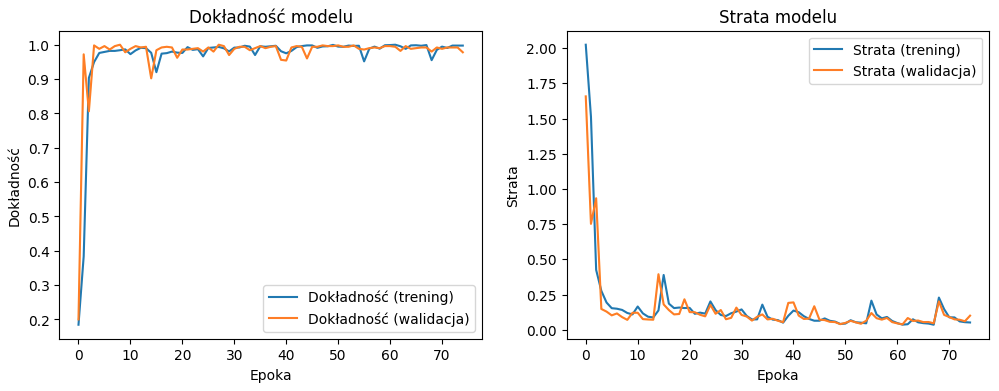
\includegraphics[height=5.5cm]{resources/tests/images/v2/multiple_edges_img.png}
	\caption{Wyniki testów dla modelu ze zmienną liczbą wierzchołków i stałą krzywizną wierzechołków}
	\label{Fig:tests-var-1}
\end{figure}
\FloatBarrier

\begin{figure}[ht]
	\centering
	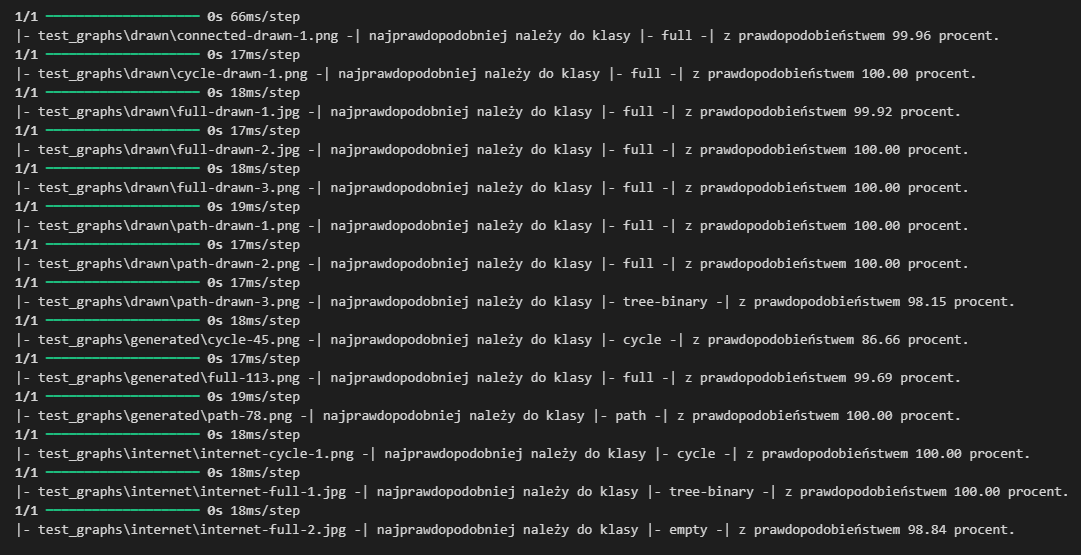
\includegraphics[height=7cm]{resources/tests/images/v2/multiple_edges_txt.png}
	\caption{Klasyfikacja obrazów zewnętrznych dla modelu z walidacją krzyżową i stałą krzywizną wierzechołków}
	\label{Fig:tests-var-2}
\end{figure}
\FloatBarrier

\textbf{Model uczony na losowej krzywiźnie wierzechołków}

Najlepsze wyniki pod względem rozpoznawania zewnętrznych obrazków testowych
oraz realistycznej dokładności na zbiorze walidacyjnym,
zostały uzyskane przy użyciu modelu sieci neuronowej uczonej na rysunkach grafów z różną liczbą wierzchołków.
Było to odpowiednio 4, 5, 6 oraz 7 wierzchołków.

\begin{figure}[ht]
	\centering
	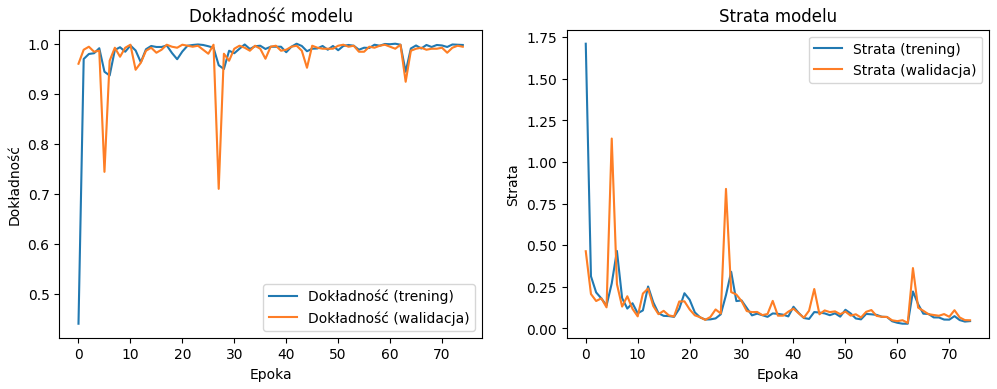
\includegraphics[height=5.5cm]{resources/tests/images/v3/multiple_edges_img.png}
	\caption{Wyniki testów dla modelu ze zmienną liczbą wierzchołków i losową krzywizną wierzchołków}
	\label{Fig:tests-var-1}
\end{figure}
\FloatBarrier

Model nie poradził sobie zbyt dobrze z obrazami zewnętrznymi, lecz znacznie lepiej niż model z walidacją krzyżową.
Poprawnie wskazanych klas grafów było 5 z 14 wszystkich rysunków.
Mimo, że model jest w stanie poprawnie określić niektóre typy grafów poprawnie,
wciąż jest to dokładność niższa niż 50\%.

\begin{figure}[ht]
	\centering
	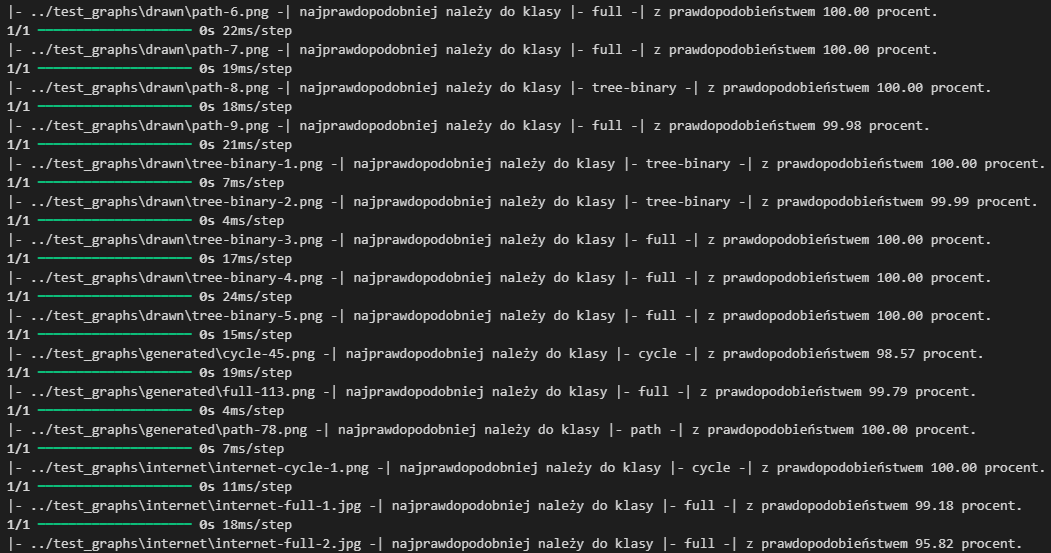
\includegraphics[height=7cm]{resources/tests/images/v3/multiple_edges_txt.png}
	\caption{Klasyfikacja obrazów zewnętrznych dla modelu z walidacją krzyżową i losową krzywizną wierzchołków}
	\label{Fig:tests-var-2}
\end{figure}
\FloatBarrier